\section{Arquitectura y diseño.}
\label{sec:arquitectura_y_diseno}

\subsection{Arquitectura.}

\subsubsection{Prácticas recomendadas por Google.}

El desarrollo de aplicaciones Android modernas requiere de una arquitectura clara, modular y escalable, que facilite el mantenimiento del código, la incorporación de nuevas funcionalidades, así como la mejora continua del producto final. Google establece principios fundamentales para el desarrollo de aplicaciones Android robustas y mantenibles a través de la plataforma Android Jetpack \cite{Jetpack}, que han evolucionado a partir de años de experiencia en el ecosistema móvil. Estas prácticas se centran en la separación clara de responsabilidades a través de una \textit{arquitectura basada en capas}, donde cada componente del sistema tiene un propósito específico y bien definido \cite{AndroidBestPractices}. 

La arquitectura recomendada para aplicaciones Android se basa principalmente en tres capas fundamentales:


\begin{itemize}
  \item \textbf{Capa de Presentación (UI):} Encargada exclusivamente de la interacción visual y la experiencia del usuario. Esta capa se ocupa de mostrar la información, escuchar las acciones del usuario y reaccionar a los cambios en el estado de la aplicación. No contiene lógica de negocio ni interacción directa con fuentes de datos, garantizando así una clara separación de responsabilidades.

  \item \textbf{Capa de Dominio (opcional, pero recomendada en proyectos de mediana o gran escala):} Constituye el núcleo lógico del sistema, implementando casos de uso específicos relacionados directamente con las reglas del negocio. Al aislar esta lógica en una capa independiente, se favorece la reutilización de código, la claridad en la implementación y se simplifican significativamente las pruebas unitarias.

  \item \textbf{Capa de Datos:} Responsable de acceder a las fuentes de información, tanto locales como remotas. Utiliza patrones de diseño como el repositorio, el cual se encarga de gestionar una fuente única de verdad para los datos, manteniendo copias locales y actualizando la información desde fuentes externas según sea necesario.
\end{itemize}

Dentro de estas prácticas es especialmente importante destacar el patrón conocido como Flujo Unidireccional de Datos \textit{(Unidirectional Data Flow, UDF)}. En el contexto específico de Android, los datos generalmente fluyen desde elementos con un alcance amplio, como los repositorios y fuentes de datos, hacia elementos con un alcance más limitado, como los componentes visuales de la UI. Por otro lado, los eventos generados por el usuario, como pulsaciones de botones o gestos, fluyen en sentido contrario desde la interfaz gráfica hacia la fuente única de verdad, donde los datos se modifican y actualizan posteriormente, siempre a través de estructuras de datos inmutables.

Este enfoque está estrechamente relacionado con la correcta gestión del ciclo de vida de los componentes Android. El conocimiento explícito y el manejo consciente del ciclo de vida permiten que los componentes reaccionen apropiadamente frente a eventos generados por el propio sistema operativo, como la rotación de pantalla o la suspensión temporal de la aplicación. Herramientas proporcionadas por Android Jetpack, como \textit{ViewModel}, y bibliotecas reactivas como \textit{LiveData} o \textit{Flow}, son clave en este proceso, pues reaccionan de forma automática y segura a los cambios de estado en las actividades y fragmentos.

Google también recomienda emplear bibliotecas especializadas como \textit{Hilt}, para gestionar las dependencias entre componentes. La inyección de dependencias automatiza la creación de objetos en tiempo de compilación sin necesidad de que cada clase los construya. En su lugar, una clase externa se encarga de proveer las dependencias requeridas, lo que simplifica la gestión de dependencias, centraliza las instancias de los objetos y mejora la mantenibilidad del código.


\subsubsection{Patrón de arquitectura MVVM.}

El patrón de arquitectura elegido para el desarrollo del launcher fue \textit{Model-View-ViewModel} (\textit{MVVM}, por sus siglas en inglés), ya que su principal objetivo es separar la lógica de negocio de la interfaz de usuario, obedeciendo a las prácticas recomendadas por Google para el desarrollo de aplicaciones Android \cite{AndroidBestPractices}. Aunque originalmente fue diseñado por Microsoft en 2005 para aplicaciones de escritorio basadas en eventos, con el tiempo ha sido cada vez más implementado en el desarrollo de aplicaciones móviles, especialmente con la introducción de \textit{Android Architecture Components} en la conferencia de Google I/O en 2017 \cite{ArchitectureComponents}. Está inspirado en el patrón \textit{Model-View-Presenter} (\textit{MVP}) y \textit{Model-View-Controller} (\textit{MVC}), manteniendo la separación de responsabilidades e introduciendo un enfoque más reactivo y menos acoplado entre la vista y el modelo. Las principales diferencias entre estos patrones arquitectónicos se presentan en la Tabla \ref{tab:comparacion_arquitecturas}.

\begin{table}[ht]
\centering
\caption{Comparación de patrones arquitectónicos: MVC, MVP y MVVM}
\label{tab:comparacion_arquitecturas}
\begin{tabular}{|p{0.2\textwidth}|p{0.25\textwidth}|p{0.25\textwidth}|p{0.25\textwidth}|}
\hline
\textbf{Aspecto} & \textbf{MVC (Model-View-Controller)} & \textbf{MVP (Model-View-Presenter)} & \textbf{MVVM (Model-View-ViewModel)} \\
\hline
\textbf{Acoplamiento} & View y Model están acoplados. Controller gestiona la interacción. & View y Model están completamente desacoplados por el Presenter. & View y ViewModel están débilmente acoplados a través de enlaces de datos (data binding). \\
\hline
\textbf{Rol de View} & Activa. Puede observar directamente a Model y recibir actualizaciones de Controller. & Pasiva. Implementa una interfaz y no contiene lógica. Presenter indica qué mostrar. & Reactiva. Se enlaza a propiedades de ViewModel y se actualiza automáticamente. \\
\hline
\textbf{Comunicación} & Controller manipula el Modelo. View puede observar al Modelo directamente. & View delega los eventos a Presenter. Presenter actualiza a View a través de una interfaz. & View se suscribe a los flujos de datos de ViewModel. Los eventos de View ejecutan funciones en el ViewModel. \\
\hline
\textbf{Referencia a View} & Controller tiene una referencia directa a View. & Presenter tiene una referencia a View, pero a través de una interfaz abstracta. & ViewModel no tiene ninguna referencia a View. La comunicación es unidireccional (View observa a ViewModel). \\
\hline
\textbf{Testabilidad} & Difícil de probar de forma aislada debido al acoplamiento entre View y Controller. & Alta. Presenter es independiente de la UI de Android y se puede probar fácilmente con mocks. & Muy alta. ViewModel es completamente independiente de View, lo que facilita las pruebas unitarias. \\
\hline
\end{tabular}
\end{table}

El patrón MVVM se compone de tres componentes principales:

\begin{itemize}
  \item \textbf{Model:} Representa la lógica de negocio y los datos de la aplicación. En el launcher, Model incluye las clases que gestionan las tareas, hábitos, límites y preferencias del usuario.

  \item \textbf{View:} Es la interfaz de usuario que muestra los datos al usuario y recibe sus interacciones. Esta capa está implementada utilizando Jetpack Compose.

  \item \textbf{ViewModel:} Actúa como un intermediario entre Model y View. Contiene la lógica para preparar los datos que View necesita y maneja las interacciones del usuario. En el launcher, cada funcionalidad principal (tareas, hábitos, limites y preferencias) tiene su propio ViewModel.
\end{itemize}

\pagebreak

El flujo de datos en MVVM es unidireccional, lo que significa que View observa los cambios en el ViewModel y se actualiza automáticamente cuando los datos cambian. Esto se logra mediante el uso de bibliotecas reactivas como \textit{Flow}, que permite a View suscribirse a los cambios en los datos y reaccionar a ellos sin necesidad de acoplarse directamente a Model. La figura \ref{fig:arquitectura_mvvm} ilustra la relación entre estos componentes.

\begin{figure}[ht]
  \caption{Arquitectura MVVM.}
  \label{fig:arquitectura_mvvm}
  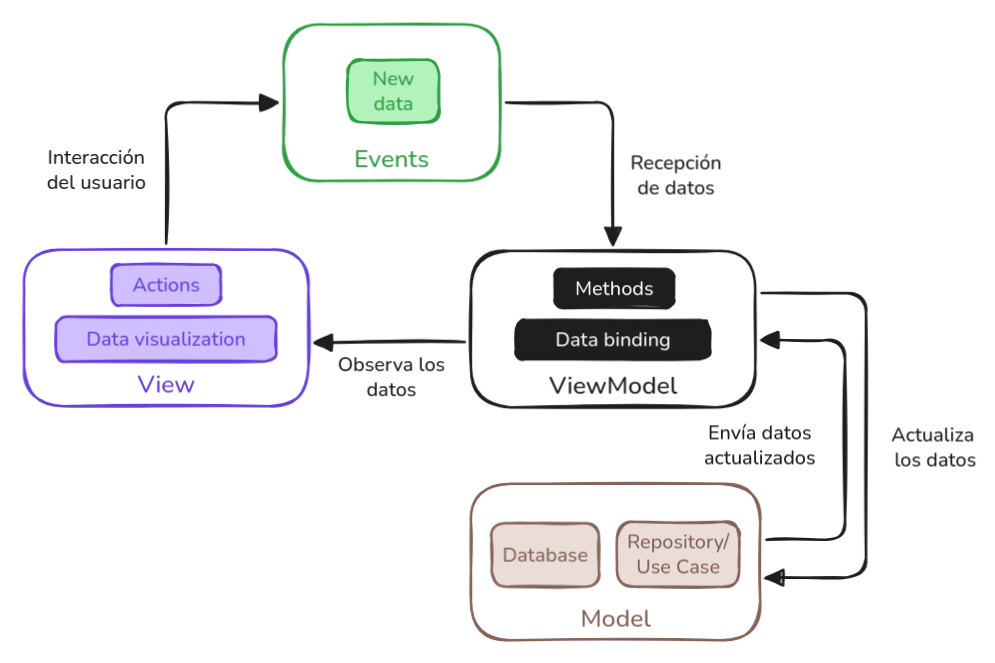
\includegraphics[width=\textwidth]{Figuras/arquitectura_mvvm.png}
  \centering
\end{figure}

\pagebreak
